\specialsection{Community}{}{black}{white}

\begin{figure}
	\centering
	\includegraphics[width=1.0\textwidth]{images/alpha-browser.png}
	\caption{Screenshot of the Processing Alpha Forum}
	\label{fig:processing-alpha}
\end{figure}

\subsection{A community of practice}
\todo[inline]{Add this in afterwards}

In this chapter, we delve into the intricate dynamics of the Processing community, a collective characterized by its collaborative ethos and commitment to open-source principles in software development. Our analysis is anchored in Wegner's Communities of Practice (CoP) model, a framework that emphasizes shared learning, mutual engagement, and the organic evolution of communal knowledge. The Processing community, with its unique blend of artists, designers, educators, and developers, presents a compelling case study for applying this model. This chapter aims to explore how the CoP model illuminates the inner workings of the Processing community, shedding light on the communal learning processes, knowledge sharing practices, and the overall evolution of this vibrant collective.

The rationale for employing Wegner's CoP model in our analysis stems from its emphasis on learning as a communal process, a concept deeply resonant with the ethos of the Processing community. This community, known for its open-source environment, thrives on peer-to-peer interaction, collaborative problem-solving, and shared creative exploration. These characteristics align closely with the three fundamental elements of Wegner's model: mutual engagement, joint enterprise, and shared repertoire. By applying this framework, we seek to understand how members of the Processing community engage with one another, contribute to shared goals, and develop a collective body of knowledge and practices. This perspective is particularly relevant in exploring how informal learning and community-driven innovation foster skill development and creativity within the Processing ecosystem.

Moreover, analyzing the Processing community through the lens of the CoP model offers valuable insights into the broader implications of community-led software development and learning. This approach allows us to go beyond the technical aspects of software creation, delving into the social dynamics and learning processes that underpin the community's success. As such, this chapter not only contributes to a deeper understanding of the Processing community itself but also provides broader lessons on the formation, sustainability, and evolution of collaborative, learning-oriented communities in the digital age. Our exploration here aims to bridge the gap between theoretical constructs and practical applications, offering both a detailed case study and a reflective consideration of the CoP model's relevance and adaptability in the context of contemporary, technology-driven communities.

% Data analysis - complement other interviews
The Alpha forum was subjected to data scraping and a preliminary analysis. This process was instrumental in identifying active members for potential interviews. The forum’s significance, as underscored by Reas, was a key consideration in this analysis. Reas asserted that the forum cultivated a ‘unified international community’ from 2002 to 2006 \parencite[331]{conradGraphicDesignPostdigital2021}, further highlighting its importance. This exploration provides valuable insights into the early stages of the Processing project and its community dynamics.

% Methodology - selecting the most active forum participants
Following an analysis of the data, the most active members by the number of posts were selected for interview, namely Ariel Malka (arielm), Martin Gomez (Martin), and Jacob Schwartz (benelek). These individuals were selected for their active participation in the forum, without being a library contributor or a core developer. A common trait amoung these people, coming from the interviews was the fact that they didn't have any graphics programming skills before participating in the forums. 



\subsection{Forum Contributors}
% Community platform should be one place of analysis
% Compare the profile of forum contributors with the profile of core contributors and library contributors
\subsection{Community Discussion Platforms}
\changepapersize{305.3mm:210mm}
\customtag{largepage}

% \setlength{\spiralWidth}{10.7mm}
% 147.3
\begin{minipage}{147.3mm}
{
	\LARGE
	\noindent Community connectedness \par
}
\begin{figure}[H]
	\centering
	\includesvg[pretex=\sffamily\fontsize{5.58pt}{8pt}\selectfont, width=1\textwidth, keepaspectratio]{images/year.svg}
	\caption{Connectedness through forum threads of top 100 alpha forum contributos}
	\label{figure:year}
\end{figure}
\end{minipage}

\newpage
\customtag{largepage}
\begin{minipage}[t]{0.7\textwidth}
\begin{figure}[H]
  \begin{adjustbox}{width=\textwidth, keepaspectratio}
      \begin{tabular}{cccc}
          % Row 1
          \begin{subfigure}[b]{0.24\textwidth}
              \centering
              \includesvg[width=\linewidth, keepaspectratio]{images/month1.svg}
              \caption{Month 1}
              \label{fig:month1}
          \end{subfigure} &
          \begin{subfigure}[b]{0.24\textwidth}
              \centering
              \includesvg[width=\linewidth, keepaspectratio]{images/month2.svg}
              \caption{Month 2}
              \label{fig:month2}
          \end{subfigure} &
          \begin{subfigure}[b]{0.24\textwidth}
              \centering
              \includesvg[width=\linewidth, keepaspectratio]{images/month3.svg}
              \caption{Month 3}
              \label{fig:month3}
          \end{subfigure} &
          \begin{subfigure}[b]{0.24\textwidth}
              \centering
              \includesvg[width=\linewidth, keepaspectratio]{images/month4.svg}
              \caption{Month 4}
              \label{fig:month4}
          \end{subfigure} \\
          % Row 2
          \begin{subfigure}[b]{0.24\textwidth}
              \centering
              \includesvg[width=\linewidth, keepaspectratio]{images/month5.svg}
              \caption{Month 5}
              \label{fig:month5}
          \end{subfigure} &
          \begin{subfigure}[b]{0.24\textwidth}
              \centering
              \includesvg[width=\linewidth, keepaspectratio]{images/month6.svg}
              \caption{Month 6}
              \label{fig:month6}
          \end{subfigure} &
          \begin{subfigure}[b]{0.24\textwidth}
              \centering
              \includesvg[width=\linewidth, keepaspectratio]{images/month7.svg}
              \caption{Month 7}
              \label{fig:month7}
          \end{subfigure} &
          \begin{subfigure}[b]{0.24\textwidth}
              \centering
              \includesvg[width=\linewidth, keepaspectratio]{images/month8.svg}
              \caption{Month 8}
              \label{fig:month8}
          \end{subfigure} \\
          % Row 3
          \begin{subfigure}[b]{0.24\textwidth}
              \centering
              \includesvg[width=\linewidth, keepaspectratio]{images/month9.svg}
              \caption{Month 9}
              \label{fig:month9}
          \end{subfigure} &
          \begin{subfigure}[b]{0.24\textwidth}
              \centering
              \includesvg[width=\linewidth, keepaspectratio]{images/month10.svg}
              \caption{Month 10}
              \label{fig:month10}
          \end{subfigure} &
          \begin{subfigure}[b]{0.24\textwidth}
              \centering
              \includesvg[width=\linewidth, keepaspectratio]{images/month11.svg}
              \caption{Month 11}
              \label{fig:month11}
          \end{subfigure} &
          \begin{subfigure}[b]{0.24\textwidth}
              \centering
              \includesvg[width=\linewidth, keepaspectratio]{images/month12.svg}
              \caption{Month 12}
              \label{fig:month12}
          \end{subfigure}
      \end{tabular}
  \end{adjustbox}
  \caption{First year of the Alpha forum}
  \label{fig:monthlyGraphs}
\end{figure}
\end{minipage}
\hfill
\begin{minipage}[t]{0.25\textwidth}
  \vspace{8mm}
  \small
  The Alpha forum's developmental trajectory over its first year, as visualized through network graphs, reveals a dynamic growth narrative. Initially, a compact hub of activity signals robust engagement from a committed group of participants, laying the groundwork for the community's expansion. This is evidenced by an increase in the density and reach of interactions, suggesting a broadening in the diversity of contributors and a rise in active membership. The persistent complexity of the network and uniform distribution of connections throughout the year highlight an environment where individuals are actively integrated, promoting a collective and inclusive exchange of knowledge.

  \medskip
  The absence of isolated clusters within these visualizations speaks to a forum culture that successfully assimilates newcomers into the ongoing dialogue, maintaining an equitable and collaborative discourse. The sustained, dense web of communications not only illustrates the forum's ability to foster long-term participant engagement but also underscores its role as a vibrant, cooperative learning space. This enduring interactivity, coupled with a consistent influx of diverse perspectives, underscores the forum's efficacy as a thriving digital ecosystem conducive to sustained collaboration and intellectual exchange.

\end{minipage}

\defaultareasettings

%\begin{figure}[h!] 
    \centering 
    \includesvg[pretex=\sffamily\fontsize{5.58pt}{8pt}\selectfont, width=1\textwidth, keepaspectratio]{images/figure-forum-posts.svg}
    \caption{Top 12 authors by number of posts (Aggregated alpha and beta forum)}
    \label{fig:forum-posts}  
  \end{figure}
%\begin{figure}[htbp] 
    \centering
    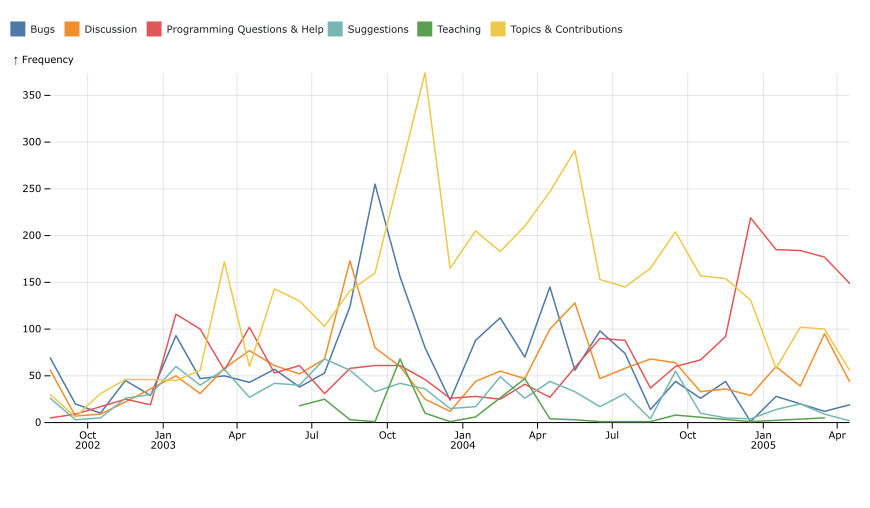
\includegraphics[width=1\textwidth]{alpha-forums-activity.png} 
    % \includesvg[pretex=\sffamily\fontsize{5.58pt}{8pt}\selectfont, width=0.6\textwidth]{images/alpha-forums-activity.svg}
    \caption{Forums activity}
    \label{fig:forum-activity}  
  \end{figure}
%\begin{figure}[h!] 
    \centering 
    \includesvg[pretex=\sffamily\fontsize{5.58pt}{8pt}\selectfont, width=1\textwidth, keepaspectratio]{images/figure-alltime-sourcecode-commits.svg}
    \caption{Top 25 source code contributors by number of commits}
    \label{fig:alltime-sourcecode-commits}  
  \end{figure}
%\begin{figure}[htbp] 
    \centering
    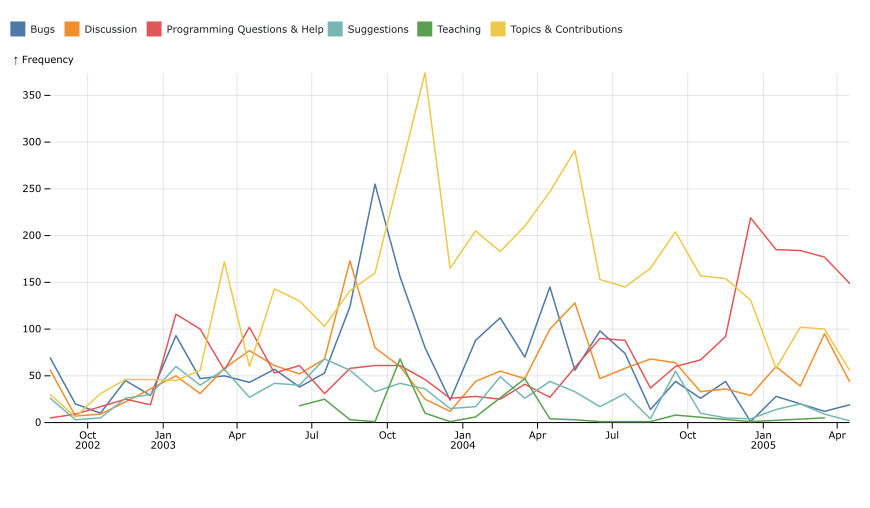
\includegraphics[width=1\textwidth]{alpha-forums-activity.png} 
    % \includesvg[pretex=\sffamily\fontsize{5.58pt}{8pt}\selectfont, width=0.6\textwidth]{images/alpha-forums-activity.svg}
    \caption{Forums activity}
    \label{fig:forum-activity}  
  \end{figure}

% \subsubsection{Alpha Forum Patterns in Forum Contributions (to remove)}
\begin{figure}[h!] 
    \centering 
    \includesvg[pretex=\sffamily\fontsize{5.58pt}{8pt}\selectfont, width=1\textwidth, keepaspectratio]{images/alpha-forums-by-posts.svg}
    \caption{Forums by number of posts}
    \label{fig:forums}  
  \end{figure}

\input{includes/processing-forums.tex}
% Interviews
% Library and code contributors
% graph of the alpha forum contributors

\newpage
\begin{figure}
	\centering
	\includegraphics[width=1.0\textwidth]{images/exhibitions.png}
	\caption{Screenshot of community exhibition}
	\label{fig:website-exhibition}
\end{figure}

\subsection{Elements of Community Engagement}
Casey Reas had an imporant role in the online community

The Processing community quickly became known for its use of examples and showcasing members' work on the exhibition page of the website. This approach not only encouraged users to share their code but also fostered a sense of community and inspiration. The initial projects published by Fry and Reas were instrumental in this regard, serving as examples that sparked discussions in the forums and fueled further interest in Processing. The community's culture of sharing and inspiration will be further explored, with specific examples such as Ariel Malka's comment on the motivation behind chronotext (\todo[inline]{Mention Ariel Malka's comment on chronotext motivation}) and the mention of Glen Murphy's work influencing Ricard Marxer (\todo[inline]{Mention of Glen Murphy's work for Ricard Marxer}). Additionally, insights from Ben Fry on how this dynamics fostered community growth will be included (\todo[inline]{Ben Fry comment on the dynamics of this fostering growth}).

Education was a cornerstone in the community's evolution. The visibility of Processing in academic settings, highlighted through classes and workshops, was significant. The connection to academia was further strengthened by Reas' teaching role, with the materials developed for Design By Numbers courses proving beneficial. This aspect will be elaborated with specific references to the involvement of educational institutions (\todo[inline]{Mention toxi comment about how schools got involved}).

The community's welcoming and friendly tone was another key factor in its success. The anonymity provided by forum usernames helped mitigate feelings of exclusion, allowing members to engage freely and look up to those making significant contributions in their fields. This inclusive atmosphere will be further detailed, including a note from Ariel Malka (\todo[inline]{Add Ariel Malka note here}).

Friendly community
Other mechanisms like Processing Community Days, Google Summer of Code, and fellowships also played a role in expanding the community's reach and impact.

\subsection{Processing Foundation}

The Processing Foundation was established in 2012 by Casey Reas, Ben Fry, and Daniel Shiffman with the primary objective of sustaining the software's development and broadening its reach. According to Fry and Reas, ``The vast majority of the code is written by the same small number of people volunteering their time — there are no paid full-time developers'' \parencite[p.~13]{fryModernPrometheusHistory2018}.

\begin{figure}[h]
	\centering
	\includegraphics[width=0.9\textwidth]{images/foundation-finances.png}
	\caption{Financial growth of the Processing Foundation over the years Source: \parencite{ProcessingFoundationNonprofit2013}}
	\label{fig:foundation-finances}
\end{figure}

As shown in Figure~\ref{fig:foundation-finances}, the foundation's revenue has experienced modest growth, increasing from \$11,235 to \$273,520. Remarkably, it reached a peak revenue of \$10,889,998 in the fiscal year 2021. Throughout its history, the principal source of funding for the foundation has predominantly come from contributions.

However, the allocation of these funds has been a point of contention within the organization. Most notably, a public disagreement in 2023 led to the resignation of Ben Fry, a long-standing board member and contributor. It should be noted that Fry's perspective on the matter was not universally accepted among the foundation's other founding members. \parencite{benfry[@ben_fry]HaveMadeExtremely2023} \parencite{caseyreas[@reas]EarlierThisWeek2023} \parencite{danielshiffman[@shiffman]WouldPostNote2023}

